% $Id: introduction.tex 87303 2016-02-08 13:44:29Z lafferty $
\begin{savequote}[8cm]
\textlatin{Neque porro quisquam est qui dolorem ipsum quia dolor sit amet, consectetur, adipisci velit...}

There is no one who loves pain itself, who seeks after it and wants to have it, simply because it is pain...
  \qauthor{--- Cicero's \textit{de Finibus Bonorum et Malorum}}
\end{savequote}

\chapter{\label{ch:2-background}\CP violation and measurements of CKM angle \Pgamma} 

\minitoc

\section{The Standard Model}

The Standard Model (SM) of particle physics describes all known fundamental particles and their interactions. Its predictions have been rigourously tested over several decades and have found to be consistent with our observations to remarkable levels of precision. Although the SM has proven to be extremely accurate it has several limitations, for example the model does not incorportate gravitational interactions, provide a dark matter candidate, or explain the huge asymmetry observed between matter and antimatter. These problems suggest that the SM is an incomplete theory, hence experimental particle physics is driven by the search for direct or indirect signs of New Physics (NP).

The SM contains twelve spin-1/2 fermions in three generations, which are grouped in quarks and leptons, listed in Table \ref{SMfermions}. These fermions interact via the electromagnetic, weak and strong forces, which are mediated by gauge bosons listed in Table \ref{SMbosons}. The Higgs boson ($H$) is the only elementary scalar particle, and it couples to all particle with mass. The Higgs mechanism explains why weak gauge bosons have mass, while the photon is massless. All these elementary particles have corresponding antiparticles. 

\begin{table}
\centering
\begin{tabular}{c|cc|cc}
& \multicolumn{2}{p{6cm}}{\hspace{2.2cm} Quarks} & \multicolumn{2}{p{6cm}}{\hspace{2.2cm} Leptons} \\
& Flavour & Charge & Flavour & Charge \\
\hline \hline
First generation & up (\uquark) & $+2/3$ & electron (e) & $-1$ \\
 & down (\dquark) & $-1/3$ & electron neutrino (\neue) & $0$ \\
\hline
Second generation & charm (\cquark) & $+2/3$ & muon (\muon) & $-1$ \\
 & strange (\squark) & $-1/3$ & muon neutrino (\neum) & $0$ \\
\hline
Third generation & top (\tquark) & $+2/3$ & tau (\tauon) & $-1$ \\
 & bottom (\bquark) & $-1/3$ & tau neutrino (\neut) & $0$ \\
\end{tabular}
\caption{Quarks and leptons in the Standard Model.}
\label{SMfermions}
\end{table}

\begin{table}
\centering
\begin{tabular}{c|cc}
Gauge boson & Force & Charge \\
\hline
photon (\g) & Electromagnetic & $0$ \\
\Z & Weak & $0$ \\
\Wpm & Weak & $\pm 1$ \\
gluon ($g$) & Strong & $0$
\end{tabular}
\caption{Gauge bosons in the Standard Model.}
\label{SMbosons}
\end{table}

\section{\CP violation}

One of the key problems with the SM is that is does not explain why our universe is matter-dominated, with hardly any antimatter present. This asymmetry is commonly quantified by the baryon-antibaryon asymmetry, $\frac{n_{B} - n_{\bar{B}}}{n_{\g}} \approx \frac{n_{B}}{n_{\g}}$, where $n_{B}$, $n_{\bar{B}}$ and $n_{\g}$ are the baryon, anti-baryon and photon number densities respectively. Astrophysical observations have measured the baryon-antibaryon asymmetry to be of the order of $10^{-10}$. The requirements for this asymmetry to be generated from a symmetrical initial state, known as baryogenisis, were first proposed by Andrei Sakarov in 1967. These three Sarkarov conditions are: baryon number violation, the violation of charge ($C$) symmetry and charge-parity (\CP) symmetry, and departure from thermal equilibrium. These components are required in all baryogenisis models. The definitions of the $C$ and $P$ symmetries are given by their operators:
\begin{itemize}
\item The charge conjugation operator, $\hat{C}$, converts particles into their antiparticles.
\item The parity operator, $\hat{P}$, reverse the spacial axis so all vectors change sign.
\end{itemize}
\CP symmetry is violated if the system changed under the combined $\hat{C}\hat{P}$ transformation.

The SM satisfies all necessary conditions for baryogenisis, however the amount of asymmetry that can be generated from \CP violation in the SM is many orders of magnitude smaller than the asymmtetry observed from astrophysical observations. New Physics models that introduce new sources of \CP violation, such as supersymmetic models, can be developed and searched for at the LHC and other experiments. However, it is also necessary to make precise measurements of \CP violation in the SM to improve our understanding of matter-antimatter asymmetry and search for indirect signs of New Physics.


\section{The CKM matrix}

Quarks in the Standard Model can interact via the strong, weak or electromagnetic interactions. For the weak interactions of the quarks, the eigenstates that take part in the W boson mediated interaction (weak eigenstates) are different to the flavour eigenstates that hadronise to produce the observable meson states \eg\ a \Bm-meson consists of \uquarkbar\bquark. The Cabibo-Kobayashi-Maskawa (CKM) matrix, given in \eqn \ref{CKMmatrix}, describes the relationship between the weak eigenstates ($d'$, $s'$, $b'$) and flavour eigenstates (\dquark, \squark, \bquark) of the quarks. 
\begin{equation}
\left(
\begin{array}{c} d' \\ s' \\ b'  \end{array} \right) =
\begin{pmatrix} V_{ud} & V_{us} & V_{ub} \\ V_{cd} & V_{cs} & V_{cb} \\ V_{td} & V_{ts} & V_{tb} \end{pmatrix} \left( 
\begin{array}{c} d \\ s \\ b \end{array} \right)
\label{CKMmatrix}
\end{equation}
The elements of this matrix, $V_{ij}$, define the coupling of a $j \to i$ quark transition. Similarly $V_{ij}^*$ defined the coupling of a $\bar{j} \to \bar{i}$ antiquark transition. By definition the CKM matrix is unitary, i.e. $V_{CKM}V_{CKM}^* = \mathds{1}$, assuming there are only three generations of quarks. The CKM matrix is a complex, $3 \times 3$ matrix, which yields 18 parameters. The unitarity requirements brings the number of free parameters down to nine. Each of the five strong phases can be redefined, leaving four free parameters: three amplitudes and one phase. This free phase parameter is the source of \CP violation in the SM.

If the CKM matrix was equivalent to the identity matrix there would be no cross-generation weak interaction of the quarks \eg\ a \uquark quark transition mediated by a W boson could only result in a \dquark, not a \squark or \bquark quark. From empirical determination, the magnitude of the elements in the CKM matrix are:
\begin{equation}
| V_{CKM} | = \begin{pmatrix} 0.97434^{+0.00011}_{0.00012} & 0.22506 \pm 0.00050 & 0.00357 \pm 0.00015 \\ 0.22492 \pm 0.00050 & 0.97351 \pm 0.00013 & 0.0411 \pm 0.0013 \\ 0.00875^{+0.00032}_{-0.00033} & 0.0403 \pm 0.0013 & 0.99915 \pm 0.00005 \end{pmatrix}
\end{equation}
It can be seen that quark transitions within the same generation is highly favoured, these are known as Cabbibo-favoured decays. Also, quark transitions across one generation are suppressed, and are even more suppressed across two generations. These are known as Cabibbo-suppressed transitions.

\section{The CKM unitarity triangle}

The unitarity of the CKM matrix leads to nine unitarity conditions, for example $\Vud\Vubs + \Vcd\Vcbs + \Vtd\Vtbs = 0$. These relations can be represented as a triangle in the complex plane. The traingle representing the condition $\Vud\Vubs + \Vcd\Vcbs + \Vtd\Vtbs = 0$ is the most used as it has sides of a similar length to each other; it has angles $\alpha$, $\beta$ and \Pgamma, and an area proportional to the amount of \CP violation in the quark sector of the Standard Model~\cite{CKMtriangle}. Overconstraining this unitarity triangle may lead to signs of physics beyond the Standard Model. The CKM angle $\Pgamma \equiv \arg\left(-\frac{\Vud{\Vub}^*}{\Vcd{\Vcb}^*}\right)$ is the least well-known angle of the CKM unitarity triangle.

The latest published \lhcb combination from direct measurements with charged and neutral \B decays to a \D meson (reconstructed in one of a variety of final states) and a kaon is $\Pgamma = \left(72.2^{+6.8}_{-7.3}\right)^{\circ}$~\cite{LHCb-PAPER-2016-032}. A global fit to the CKM triangle by the CKMfitter group~\cite{CKMFitter}, shown in \fig\ref{globalfit}, obtains a \Pgamma value of $(66.9^{+0.9}_{-3.4})^{\circ}$, where this determination of \Pgamma excludes all direct measurements. The uncertainties on the indirect measurement are expected to decrease as lattice QCD calculations become more accurate. Therefore, precision at the level of $1^\circ$ on a direct measurement of \Pgamma would test the consistency of the direct and indirect measurements and thereby the Standard Model. This precision can be achieved through a combination of measurements of various \B decays that are sensitive to \Pgamma.

\begin{figure}[!ht]
\centering
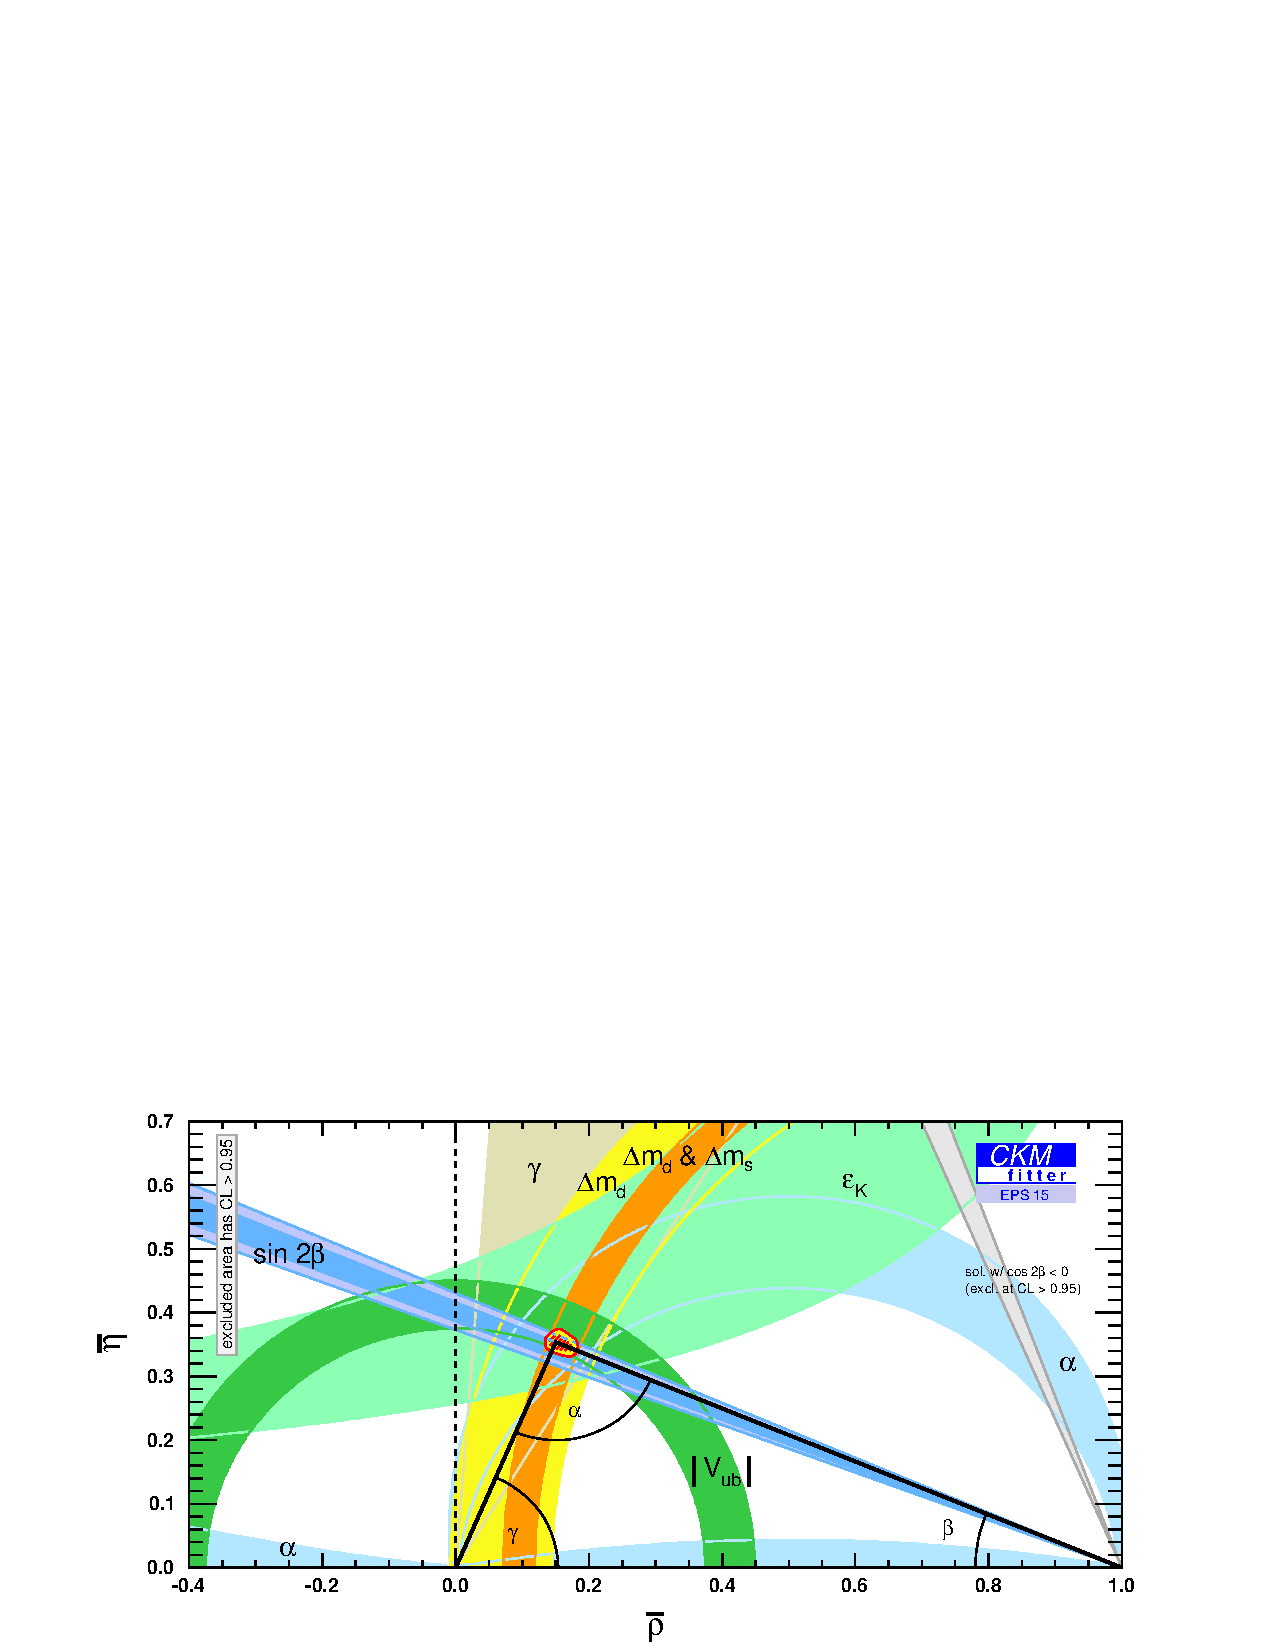
\includegraphics[trim = 0mm 0mm 0mm 180mm,clip,width=0.9\linewidth]{figures/theory/rhoeta_small_global.pdf}
\caption{Diagram showing the current state of measurements of the unitarity triangle. The black line shows the fit obtained by CKM fitter}
\label{globalfit}
\end{figure}

\section{Tree-level determination of \Pgamma using \decay{\Bpm}{\D K^{(*)\pm}} decays}

Direct measurements of \Pgamma can be made by exploiting the interference between \decay{\bquark}{\cquark\uquarkbar\squark} and \decay{\bquark}{\uquark\cquarkbar\squark} transitions. These transitions are present at tree-level in $\Bpm \to \D\kaon^{(*)\pm}$ decays, represented by the Feynman diagrams shown in \fig\ref{fig:B2DKstarmdiagram}, showing \decay{\Bm}{\Dz\Kstarm} (left) and \decay{\Bm}{\Dzb\Kstarm} (right). 
\begin{figure}[!h]
\centering
\resizebox{0.48\linewidth}{!}{
	\begin{tikzpicture}[scale=0.98]
        % MAP OUT VERTICES (I have 8 of them)
        \coordinate (a) at (0,2); %b quark start
        \coordinate (b) at (0,1); %ubar quark start
        \coordinate (c) at (5,1); %ubar quark end
        \coordinate (d) at (5,2); %c quark end
        \coordinate (e) at (2,2); %start the W+
        \coordinate (f) at (5,2.67); %s quark
        \coordinate (g) at (5,3.33); %ubar quark
        \coordinate (h) at (4.0,3); %W end
        % DRAW LINES
        \draw[antiparticle] (b)  -- (c); %ubar quark
        \draw[particle] (a)  -- (e); %bbar quark
        \draw[particle] (e)  -- (d); %ubar quark 
        \draw[photon] (e) -- (h); %W+
        \draw[antiparticle] (h)  to (g); %W to ubar quark
        \draw[particle] (h)  to (f); %W to s quark 
        %DRAW LABELS
        \node at ($(a)$) [label={[label distance=-4mm] b},left] {};
        \node at ($(b)$) [label={[label distance=-4mm] $\bar{\rm u}$},left] {};
        \node at ($(c)$) [label={[label distance=-4mm] $\bar{\rm u}$},right]{};
        \node at ($(d)$) [label={[label distance=-4mm] c},right] {};
        \node at ($(f)$) [label={[label distance=-4mm] s},right] {};
        \node at ($(g)$) [label={[label distance=-4mm] $\bar{\rm u}$},right]{};
        \node at ($(e)$) [label={[xshift=25pt,yshift=10pt] $W^-$},above] {};

        %ADD BRACES
        \draw
        [black,decorate,decoration={brace,amplitude=5pt},xshift=-20pt,yshift=0pt]
          (0,0.8)  -- (0,2.2) node [black,midway,left=0pt,xshift=-5pt]{$\Bm$};
        \draw
        [black,decorate,decoration={brace,amplitude=5pt},xshift=20pt,yshift=0pt]
          (5,3.53) -- (5,2.47) node [black,midway,right=0pt,xshift=5pt]{$\Kstarm$};
         \draw 	[black,decorate,decoration={brace,amplitude=5pt},xshift=20pt,yshift=0pt]
          (5,2.2)  -- (5,0.8) node [black,midway,right=0pt,xshift=5pt] {$\Dz$};
            \end{tikzpicture}
        }
\resizebox{0.47\linewidth}{!}{
\begin{tikzpicture}[scale=0.98]
        % MAP OUT VERTICES (I have 8 of them)
        \coordinate (a) at (0,3); %b quark start
        \coordinate (b) at (0,1); %ubar quark start
        \coordinate (c) at (5,1); %ubar quark end
        \coordinate (d) at (5,3); %u quark end
        \coordinate (e) at (2,3); %start the W+
        \coordinate (f) at (5,1.67); %s quark
        \coordinate (g) at (5,2.33); %cbar quark
        \coordinate (h) at (4.0,2); %W end
        % DRAW LINES
        \draw[antiparticle] (b)  -- (c); %ubar quark
        \draw[particle] (a)  -- (e); %b quark
        \draw[particle] (e)  -- (d); %u quark 
        \draw[photon] (e) -- (h); %W+
        \draw[antiparticle] (h)  to (g); %W to cbar quark
        \draw[particle] (h)  to (f); %W to s quark 
        %DRAW LABELS
        \node at ($(a)$) [label={[label distance=-4mm] b},left] {};
        \node at ($(b)$) [label={[label distance=-4mm] $\bar{\rm u}$},left] {};
        \node at ($(c)$) [label={[label distance=-4mm] $\bar{\rm u}$},right]{};
        \node at ($(d)$) [label={[label distance=-4mm] u},right] {};
        \node at ($(f)$) [label={[label distance=-4mm] s},right] {};
        \node at ($(g)$) [label={[label distance=-4mm] $\bar{\rm c}$},right]{};
        \node at ($(e)$) [label={[xshift=25pt,yshift=-40pt] $W^-$},above] {};

        %ADD BRACES
        \draw 	[black,decorate,decoration={brace,amplitude=5pt},xshift=-20pt,yshift=0pt]
        (0,0.8)  -- (0,3.2) node [black,midway,left=0pt,xshift=-5pt] {$\Bm$};
        \draw [black,decorate,decoration={brace,amplitude=5pt},xshift=20pt,yshift=0pt]
        (5,1.85)  -- (5,0.8) node [black,midway,right=0pt,xshift=5pt] {$\Kstarm$};
         \draw [black,decorate,decoration={brace,amplitude=5pt},xshift=20pt,yshift=0pt]
        (5,3.2)  -- (5,2.15) node [black,midway,right=0pt,xshift=5pt] {$\bar{\rm \Dz}$};
        \end{tikzpicture}
    }
    \caption{Leading order Feynman diagrams for \decay{\Bm}{\Dz\Kstarm} (left) and \decay{\Bm}{\Dzb\Kstarm} (right).}
    \label{fig:B2DKstarmdiagram}
\end{figure}
The ratio of the amplitudes between the \decay{\Bm}{\Dzb\Kstarm} decay and the \decay{\Bm}{\Dz\Kstarm} and their charge conjugates is shown in \eqn\ref{ratiodiagrams}.
\begin{equation}
\frac{\mathcal{A}\left(\decay{\Bm}{\Dzb\Kstarm}\right)}{\mathcal{A}\left(\decay{\Bm}{\Dz\Kstarm}\right)} = \rb e^{i(\deltab - \gamma)} \text{ , }
\frac{\mathcal{A}\left(\decay{\Bp}{\Dz\Kstarp}\right)}{\mathcal{A}\left(\decay{\Bp}{\Dzb\Kstarp}\right)} = \rb e^{i(\deltab + \gamma)}
\label{ratiodiagrams}
\end{equation}
There are three parameters introduced in \eqn\ref{ratiodiagrams}: \rb, \deltab and \Pgamma. The angle \Pgamma is the \CP violating weak phase angle form the CKM traingle, \rb is the magntiude of ratio of the amplitudes and \deltab is difference in strong phase between the suppressed and favoured decays.

The effect of the interference between the two diagrams in \fig\ref{fig:B2DKstarmdiagram} can be observed by reconstructing the \D meson in a final state accessible to both \Dz and \Dzb meson states, with the final state labelled $f(D)$. This interference gives sensitivity to the weak phase \Pgamma. In the following description we assume \CP violation in the charm sector is negligible, and effects of \D mixing are neglected. The ampltiudes of the \Bm and \Bp decays are given by \eqn\ref{BandDdecaysminus} and \ref{BandDdecaysplus}, where $A_D$ is the amplitude of \decay{\Dz}{f(D)} and $\bar{A_{D}}$ is the ampltiude of \decay{\Dzb}{f(D)}. The two terms in these equations correspond to the two diagrams in \fig\ref{fig:B2DKstarmdiagram}.
\begin{align}
\mathcal{A}\left(\decay{\Bm}{[f(D)]\Kstarm}\right) &= A_{D} + \bar{A_{D}}\rb e^{i(\deltab - \gamma)} \label{BandDdecaysminus} \\
\mathcal{A}\left(\decay{\Bp}{[f(D)]\Kstarp}\right) &= \bar{A_{D}} + A_{D}\rb e^{i(\deltab + \gamma)} \label{BandDdecaysplus}
\end{align}

The values of the complex amplitudes, $A_{D}$ and $\bar{A_{D}}$, depend on the \D meson final state chosen.


\subsection{The GLW method}

The GLW method~\cite{GL,GW} uses \D decay modes that are \CP eigenstates, such as the \CP-even eigenstates \decay{\D}{\Kp\Km} and \decay{\D}{\pip\pim}. As the final states are \CP eigenstates, the expressions from \eqn\ref{BandDdecaysminus} and \ref{BandDdecaysplus} can be simplified to
\begin{align}
\mathcal{A}\left(\decay{\Bm}{[f_{GLW}]\Kstarm}\right) &\propto 1 + \rb e^{i(\deltab - \gamma)} \label{glwBdecaym} \\
\mathcal{A}\left(\decay{\Bp}{[f_{GLW}]\Kstarp}\right) &\propto 1 + \rb e^{i(\deltab + \gamma)} \label{glwBdecayp}
\end{align}
assuming that \CP violation in \D decays is negligible and $\mathcal{A}\left(\decay{\Bm}{\Dz\Kstarm}\right) = \mathcal{A}\left(\decay{\Bp}{\Dzb\Kstarp}\right)$. The partial widths can be expressed as
\begin{align}
\Gamma\left(\decay{\Bm}{[f_{GLW}]\Kstarm}\right) &= \left|\mathcal{A}\left(\decay{\Bm}{[f_{GLW}]\Kstarm}\right)\right|^2 \nonumber \\
&\hspace{48pt} \propto 1 + \rb^2 + 2\rb\cos(\deltab - \gamma) \label{widthBm} \\
\Gamma\left(\decay{\Bp}{[f_{GLW}]\Kstarp}\right) &= \left| \mathcal{A}\left(\decay{\Bp}{[f_{GLW}]\Kstarp}\right)\right|^2 \nonumber \\
&\hspace{48pt} \propto 1 + \rb^2 + 2\rb\cos(\deltab + \gamma) \label{widthBp}
\end{align}
The four-body \D decay mode \decay{\D}{\pip\pim\pip\pim} is an approximate \CP eigenstate, although as it is not a pure \CP eigenstate its sensitivity to \Pgamma is reduced. The parameter $F_{4\pi} \sim 0.75$~\cite{charm4pi} is the \CP-even fraction, which accounts for the dilution effect. The corresponding equations for \ref{widthBm} and \ref{widthBp} are
\begin{align}
\Gamma\left(\decay{\Bm}{[f_{qGLW}]\Kstarm}\right) \propto 1 + \rb^2 + 2\rb\left(2F_{4\pi} - 1\right)\cos(\deltab - \gamma) \label{widthBm4body} \\
\Gamma\left(\decay{\Bp}{[f_{GLW}]\Kstarp}\right) \propto 1 + \rb^2 + 2\rb\left(2F_{4\pi} - 1\right)\cos(\deltab + \gamma) \label{widthBp4body}
\end{align}


\subsection{The ADS method}

The ADS method~\cite{ADS,ADS-2001} uses \D decay modes where $f(D)$ is a non-\CP eigenstate such as \decay{\D}{\Km\pip}. A key feature of this method is that although the \Dz and \Dzb decay to the same final state they proceed by very different amplitudes. The Feynman diagrams for the doubly Cabbibo-favoured \decay{\Dz}{\Km\pip} decay and the doubly Cabbibo-suppressed \decay{\Dzb}{\Kp\pim} decay are shown in \fig\ref{fig:D2KPidiagram}.
\begin{figure}[!h]
\centering
\resizebox{0.48\linewidth}{!}{
	\begin{tikzpicture}[scale=0.98]
        % MAP OUT VERTICES (I have 8 of them)
        \coordinate (a) at (0,2); %c quark start
        \coordinate (b) at (0,1); %ubar quark start
        \coordinate (c) at (5,1); %ubar quark end
        \coordinate (d) at (5,2); %s quark end
        \coordinate (e) at (2,2); %start the W+
        \coordinate (f) at (5,2.67); %dbar quark
        \coordinate (g) at (5,3.33); %u quark
        \coordinate (h) at (4.0,3); %W end
        % DRAW LINES
        \draw[antiparticle] (b)  -- (c); %ubar quark
        \draw[particle] (a)  -- (e); %bbar quark
        \draw[particle] (e)  -- (d); %ubar quark 
        \draw[photon] (e) -- (h); %W+
        \draw[antiparticle] (h)  to (g); %W to ubar quark
        \draw[particle] (h)  to (f); %W to s quark 
        %DRAW LABELS
        \node at ($(a)$) [label={[label distance=-4mm] c},left] {};
        \node at ($(b)$) [label={[label distance=-4mm] $\bar{\rm u}$},left] {};
        \node at ($(c)$) [label={[label distance=-4mm] $\bar{\rm u}$},right]{};
        \node at ($(d)$) [label={[label distance=-4mm] s},right] {};
        \node at ($(f)$) [label={[label distance=-4mm] $\bar{\rm d}$},right]{};
        \node at ($(g)$) [label={[label distance=-4mm] u},right]{};
        \node at ($(e)$) [label={[xshift=25pt,yshift=10pt] $W^+$},above] {};

        %ADD BRACES
        \draw
        [black,decorate,decoration={brace,amplitude=5pt},xshift=-20pt,yshift=0pt]
          (0,0.8)  -- (0,2.2) node [black,midway,left=0pt,xshift=-5pt]{\Dz};
        \draw
        [black,decorate,decoration={brace,amplitude=5pt},xshift=20pt,yshift=0pt]
          (5,3.53) -- (5,2.47) node [black,midway,right=0pt,xshift=5pt]{\pip};
         \draw 	[black,decorate,decoration={brace,amplitude=5pt},xshift=20pt,yshift=0pt]
          (5,2.2)  -- (5,0.8) node [black,midway,right=0pt,xshift=5pt] {\Km};
            \end{tikzpicture}
        }
\resizebox{0.47\linewidth}{!}{
\begin{tikzpicture}[scale=0.98]
        % MAP OUT VERTICES (I have 8 of them)
        \coordinate (a) at (0,2); %c quark start
        \coordinate (b) at (0,1); %ubar quark start
        \coordinate (c) at (5,1); %ubar quark end
        \coordinate (d) at (5,2); %d quark end
        \coordinate (e) at (2,2); %start the W+
        \coordinate (f) at (5,2.67); %u quark
        \coordinate (g) at (5,3.33); %sbar quark
        \coordinate (h) at (4.0,3); %W end
        % DRAW LINES
        \draw[antiparticle] (b)  -- (c); %ubar quark
        \draw[particle] (a)  -- (e); %bbar quark
        \draw[particle] (e)  -- (d); %ubar quark 
        \draw[photon] (e) -- (h); %W+
        \draw[antiparticle] (h)  to (g); %W to ubar quark
        \draw[particle] (h)  to (f); %W to s quark 
        %DRAW LABELS
        \node at ($(a)$) [label={[label distance=-4mm] c},left] {};
        \node at ($(b)$) [label={[label distance=-4mm] $\bar{\rm u}$},left] {};
        \node at ($(c)$) [label={[label distance=-4mm] $\bar{\rm u}$},right]{};
        \node at ($(d)$) [label={[label distance=-4mm] d},right]{};
        \node at ($(f)$) [label={[label distance=-4mm] u},right]{};
        \node at ($(g)$) [label={[label distance=-4mm] $\bar{\rm s}$},right]{};
        \node at ($(e)$) [label={[xshift=25pt,yshift=10pt] $W^+$},above] {};

        %ADD BRACES
        \draw
        [black,decorate,decoration={brace,amplitude=5pt},xshift=-20pt,yshift=0pt]
          (0,0.8)  -- (0,2.2) node [black,midway,left=0pt,xshift=-5pt]{\Dz};
        \draw
        [black,decorate,decoration={brace,amplitude=5pt},xshift=20pt,yshift=0pt]
          (5,3.53) -- (5,2.47) node [black,midway,right=0pt,xshift=5pt]{\Kp};
         \draw 	[black,decorate,decoration={brace,amplitude=5pt},xshift=20pt,yshift=0pt]
          (5,2.2)  -- (5,0.8) node [black,midway,right=0pt,xshift=5pt] {\pim};
            \end{tikzpicture}
    }
    \caption{Leading order Feynman diagrams for \decay{\Dz}{\Km\pip} (left) and \decay{\Dz}{\Kp\pim} (right).}
    \label{fig:D2KPidiagram}
\end{figure}

The ratio of the amplitude between \decay{\Dzb}{\Km\pip} and \decay{\Dz}{\Km\pip} is given in \eqn\ref{ratioads}. The parameter $r_D$ is the magntiude of ratio of the amplitudes and $\delta_D$ is difference in strong phase between the suppressed and favoured decays.
\begin{equation}
\frac{\mathcal{A}\left(\decay{\Dzb}{\Km\pip}\right)}{\mathcal{A}\left(\decay{\Dz}{\Km\pip}\right)} = r_D^{K\pi}e^{-\delta_D^{K\pi}}
\label{ratioads}
\end{equation}

The amplitudes for the various \decay{\Bpm}{\D\Kstarpm} decays with ADS decay modes. 
\begin{align}
\mathcal{A}\left(\decay{\Bm}{[\Kp\pim]\Kstarm}\right) &\propto r_D^{K\pi}e^{-\delta_D^{K\pi}} + \rb e^{i(\deltab - \gamma)} \label{adsBdecaym} \\
\mathcal{A}\left(\decay{\Bp}{[\Km\pip]\Kstarp}\right) &\propto r_D^{K\pi}e^{-\delta_D^{K\pi}} + \rb e^{i(\deltab + \gamma)} \label{adsBdecayp} \\
\mathcal{A}\left(\decay{\Bm}{[\Km\pip]\Kstarm}\right) &\propto 1 + \rb r_D^{K\pi} e^{i(\deltab - \gamma)}e^{-\delta_D^{K\pi}} \label{favBdecaym} \\
\mathcal{A}\left(\decay{\Bp}{[\Kp\pim]\Kstarp}\right) &\propto 1 + \rb r_D^{K\pi} e^{i(\deltab + \gamma)}e^{-\delta_D^{K\pi}} \label{favBdecayp} 
\end{align}
In the favoured decay, the pion from the \D meson and that from the \Kstarm meson have opposite charge, while in the suppressed decay the pion from the \D meson and that from the \Kstarm meson have the same charge. The ADS decay mode is a combination of a CKM-favoured \decay{\Bm}{\Dz\Kstarm} decay, followed by a doubly Cabibbo-suppressed \decay{\Dz}{\Kp\pim} decay, and a CKM- and colour-suppressed \decay{\Bm}{\Dzb\Kstarm} decay, followed by a Cabibbo-favoured \decay{\Dzb}{\Kp\pim} decay. Both paths to the same final state have amplitudes of similar size, and interference effects are therefore magnified in comparison to the GLW decay modes, where the decay path via the CKM-favoured \decay{\Bm}{\Dz\Kstarm} dominates.

Two-body \decay{\D}{\Kmp\pipm} decays are characterised by a single strong phase, however for multibody \decay{\D}{\Kmp\pipm\pimp\pipm} decays the strong phase varies over the phase space. By averaging the strong phase variation the interference effects are diluted, which is accounted for by the parameter $\kappa_{K3\pi}$.

\subsection{The coherence factor}

The $K^*(892)$ meson has a large natural width (about 50 MeV~\cite{PDG2016}), therefore non-resonant \decay{\Bm}{\D\KS\pim} processes may be non-neglibigle, which would affect the measurement of \Pgamma. Due to the large natural width, the amplitudes and phases of the different decays may be different at each point in phasespace:
\begin{align*}
A(B^- \to D^0 K^{*-}) &= A_c(p) e^{i\delta_c(p)} \\
A(B^- \to \bar{D^0} K^{*-}) &= A_u(p) e^{i\delta_u(p) e^{-i\gamma}} \\
A(D^0 \to K^-\pi^+) &= A_{K\pi} e^{i\delta_{K\pi}} \\
A(D^0 \to K^+\pi^-) &= A_{{\pi}K} e^{i\delta_{{\pi}K}} 
\end{align*}
\begin{align*}
r_B &= \frac{\Gamma(B^- \to \bar{D^0}K^{*-})}{\Gamma(B^- \to D^0K^{*-})} = \frac{\int \left|A_u(p)\right|^2 \mathrm{d}p}{\int \left|A_c(p)\right|^2 \mathrm{d}p}
\end{align*}
\begin{align}
\kappa e^{i\delta_B} &= \frac{\int \mathrm{d}p A_c(p)A_u(p)e^{i\delta(p)}}{\sqrt{\int \mathrm{d}p \left|A_u(p)\right|^2 \int \mathrm{d}p \left|A_c(p)\right|^2}}
\label{kappadefinition}
\end{align}
where p represents a point in phasespace, and $0 \leq \kappa \leq 1$ and $0 \leq \delta_B \leq 2\pi$. The amplitudes include both resonant $B^- \to DK^{*-}$ and non-resonant contributions, which is what the coherence factor, $\kappa$, accounts for.

Using this formalism it can be shown that the $\kappa$ factor can be included in the expressions of the CP observables as shown in Equations \ref{exp_Acp}, \ref{exp_Rcp} and \ref{exp_Rpm}. The value for $\kappa$ can be estimated and then used alongside the CP observables to extract \Pgamma, $r_B$ and $\delta_B$.

\subsection{Physical observables}

The favoured mode is used  as a control mode for many aspects of the analysis since no \CP asymmetry is expected.

Twelve quantities, collectively referred to as \CP observables, are measured in this analysis:

\begin{itemize}
\item{The \CP asymmetry for the favoured decay mode
{\footnotesize
\begin{equation}
A_{\kaon\pi} = \frac{\Gamma\left(\decay{\Bm}{\D(\Km\pip)\Kstarm}\right) - \Gamma\left(\decay{\Bp}{\D(\Kp\pim)\Kstarp}\right)}{\Gamma\left(\decay{\Bm}{\D(\Km\pip)\Kstarm}\right) + \Gamma\left(\decay{\Bp}{\D(\Kp\pim)\Kstarp}\right)} \text{ .}
\label{eqn:Akpi}
\end{equation}}%
\noindent%
This asymmetry should be essentially zero due to the very small interference expected in this configuration of \B- and \D-meson decays.
}
\item{The \CP asymmetry for the \decay{\D}{\Kp\Km} decay mode
{\footnotesize
\begin{equation}
A_{\kaon\kaon} = \frac{\Gamma\left(\decay{\Bm}{\D(\Kp\Km)\Kstarm}\right) - \Gamma\left(\decay{\Bp}{\D(\Kp\Km)\Kstarp}\right)}{\Gamma\left(\decay{\Bm}{\D(\Kp\Km)\Kstarm}\right) + \Gamma\left(\decay{\Bp}{\D(\Kp\Km)\Kstarp}\right)} \text{ . }
\label{eqn:Akk}
\end{equation}
}}
\item{The \CP asymmetry for the \decay{\D}{\pip\pim} decay mode
{\footnotesize
\begin{equation}
A_{\pi\pi} = \frac{\Gamma\left(\decay{\Bm}{\D(\pip\pim)\Kstarm}\right) - \Gamma\left(\decay{\Bp}{\D(\pip\pim)\Kstarp}\right)}{\Gamma\left(\decay{\Bm}{\D(\pip\pim)\Kstarm}\right) + \Gamma\left(\decay{\Bp}{\D(\pip\pim)\Kstarp}\right)} \text{ . }
\label{eqn:Apipi}
\end{equation}}
}
Assuming negligible direct \CP violation in \D-meson decays, the observables $A_{\kaon\kaon}$ and $A_{\pi\pi}$ should be equal and are often labelled together as $A_{CP+}$.
\item{The ratio of the rate for the \decay{\D}{\Kp\Km} decay mode to that of the favoured decay mode, scaled by the branching fractions
{\footnotesize
\begin{equation}
R_{\kaon\kaon} = \frac{\Gamma\left(\decay{\Bm}{\D(\Kp\Km)\Kstarm}\right) + \Gamma\left(\decay{\Bp}{\D(\Kp\Km)\Kstarp}\right)}{\Gamma\left(\decay{\Bm}{\D(\Km\pip)\Kstarm}\right) + \Gamma\left(\decay{\Bp}{\D(\Kp\pim)\Kstarp}\right)} \cdot \frac{\BR(D^0 \to K^-\pi^+)}{\BR(D^0 \to K^+K^-)} \text{ . }
\label{eqn:Rkk}
\end{equation}
}}
\item{The ratio of the rate for the \decay{\D}{\pip\pim} decay mode to that of the favoured decay mode, scaled by the branching fractions
{\footnotesize
\begin{equation}
R_{\pi\pi} = \frac{\Gamma\left(\decay{\Bm}{\D(\pip\pim)\Kstarm}\right) + \Gamma\left(\decay{\Bp}{\D(\pip\pim)\Kstarp}\right)}{\Gamma\left(\decay{\Bm}{\D(\Km\pip)\Kstarm}\right) + \Gamma\left(\decay{\Bp}{\D(\Kp\pim)\Kstarp}\right)} \cdot \frac{\BR(D^0 \to K^-\pi^+)}{\BR(D^0 \to \pi^+\pi^-)} \text{ . }
\label{eqn:Rpipi}
\end{equation}}
}
Assuming negligible direct \CP violation in \D-meson decays, the observables $R_{\kaon\kaon}$ and $R_{\pi\pi}$ should be equal and are often labelled together as $R_{CP+}$.
\item{The ratio of the rate for the ADS decay mode to that of the favoured decay mode for \Bp decays
{\footnotesize
\begin{equation}
R^+_{K\pi} = \frac{\Gamma\left(\decay{\Bp}{\D(\Km\pip)\Kstarp}\right)}{\Gamma\left(\decay{\Bp}{\D(\Kp\pim)\Kstarp}\right)} \text{ . }
\label{eqn:Rplus}
\end{equation}
}}
\item{The ratio of the rate for the ADS decay mode to that of the favoured decay mode for \Bm decays
{\footnotesize
\begin{equation}
R^-_{K\pi} = \frac{\Gamma\left(\decay{\Bm}{\D(\Kp\pim)\Kstarm}\right)}{\Gamma\left(\decay{\Bm}{\D(\Km\pip)\Kstarm}\right)} \text{ . }
\label{eqn:Rminus}
\end{equation}
}}
\item{The \CP asymmetry for the favoured \decay{\Dz}{\Km\pip\pim\pip} decay mode
{\footnotesize
\begin{equation}
A_{\kaon\pi\pi\pi} = \frac{\Gamma\left(\decay{\Bm}{\D(\Km\pip\pim\pip)\Kstarm}\right) - \Gamma\left(\decay{\Bp}{\D(\Kp\pim\pip\pim)\Kstarp}\right)}{\Gamma\left(\decay{\Bm}{\D(\Km\pip\pim\pip)\Kstarm}\right) + \Gamma\left(\decay{\Bp}{\D(\Kp\pim\pip\pim)\Kstarp}\right)} \text{ . }
\label{eqn:Akpipipi}
\end{equation}}%
\noindent%
This asymmetry should be essentially zero due to the very small interference expected in this configuration of \B- and \D-meson decays.
}
\item{The \CP asymmetry for the \decay{\D}{\pip\pim\pip\pim} decay mode
{\footnotesize
\begin{equation}
A_{\pi\pi\pi\pi} = \frac{\Gamma\left(\decay{\Bm}{\D(\pip\pim\pip\pim)\Kstarm}\right) - \Gamma\left(\decay{\Bp}{\D(\pip\pim\pip\pim)\Kstarp}\right)}{\Gamma\left(\decay{\Bm}{\D(\pip\pim\pip\pim)\Kstarm}\right) + \Gamma\left(\decay{\Bp}{\D(\pip\pim\pip\pim)\Kstarp}\right)} \text{ . }
\label{eqn:Apipipipi}
\end{equation}
}}
\item{The ratio of the rate for the \decay{\D}{\pip\pim\pip\pim} decay mode to that of the favoured decay mode, scaled by the branching fractions
{\footnotesize
\begin{equation}
R_{\pi\pi\pi\pi} = \frac{\Gamma\left(\decay{\Bm}{\D(\pip\pim\pip\pim)\Kstarm}\right) + \Gamma\left(\decay{\Bp}{\D(\pip\pim\pip\pim)\Kstarp}\right)}{\Gamma\left(\decay{\Bm}{\D(\Km\pip\pim\pip)\Kstarm}\right) + \Gamma\left(\decay{\Bp}{\D(\Kp\pim\pip\pim)\Kstarp}\right)} \cdot \frac{\mathcal{B}(D^0 \to \Km\pip\pim\pip)}{\mathcal{B}(D^0 \to \pip\pim\pip\pim)} \text{ . }
\label{eqn:Rpipipipi}
\end{equation}}
}
\item{The ratio of the rate for the four-body ADS decay mode to that of the four-body favoured decay mode for \Bp decays
{\footnotesize
\begin{equation}
R^+_{K\pi\pi\pi} = \frac{\Gamma\left(\decay{\Bp}{\D(\Km\pip\pim\pip)\Kstarp}\right)}{\Gamma\left(\decay{\Bp}{\D(\Kp\pim\pip\pim)\Kstarp}\right)} \text{ . }
\label{eqn:Rplus4body}
\end{equation}
}}
\item{The ratio of the rate of the four-body ADS decay mode to that of the four-body favoured decay mode for \Bm decays
{\footnotesize
\begin{equation}
R^-_{K\pi\pi\pi} = \frac{\Gamma\left(\decay{\Bm}{\D(\Kp\pim\pip\pim)\Kstarm}\right)}{\Gamma\left(\decay{\Bm}{\D(\Km\pip\pim\pip)\Kstarm}\right)} \text{ . }
\label{eqn:Rminus4body}
\end{equation}
}}
\end{itemize}

\noindent
In contrast to the GLW decay modes, for the ADS decay mode the ratios are measured separately for the positive and negative charges. These observables have statistical uncertainties that are more Gaussian than asymmetry variables for the very low yields that are expected. 

Several \CP observables measured in this analysis can be related to the physics parameters to be determined, namely \Pgamma, $r_B$, $\delta_B$ and $\kappa$. The parameter $r_B$ is the magnitude of the ratio between the suppressed and favoured amplitudes of the \B-meson decay and $\delta_B$ is the strong-phase difference between these amplitudes. The expectation value is $r_B$ $\sim 0.1$, similar to that in the \decay{\Bm}{\D\Km} decay due to the similarity of the hadronic interactions. Both $r_B$ and $\delta_B$ are averaged over the region of \D\KS\pim phase space corresponding to the \Kstarm-meson selection window. The coherence factor $\kappa$ accounts for the contribution of \CP violation from $\Bm \to D \KS \pim$ decays that are not due to an intermediate $K^*(892)^{-}$ resonance~\cite{Gronau2003198}, where $\kappa = 1$ denotes pure $K^*(892)^{-}$. Assuming a negligible effect from charm mixing~\cite{charmmixing}, the relationships between the \CP observables and physics parameters are given in the following equations,
\begin{equation}
A_{\CP+} = \frac{2 \kappa r_B\sin\delta_B\sin\gamma}{1 + r_B^2 + 2 \kappa r_B\cos\delta_B\cos\gamma}
\label{exp_Acp}
\end{equation}
\begin{equation}
R_{\CP+} = 1 + r_B^2 + 2 \kappa r_B\cos\delta_B\cos\gamma
\label{exp_Rcp}
\end{equation}
\begin{equation}
R^{\pm}_{K\pi} = \frac{r_B^2 + \left(r_D^{K\pi}\right)^2 + 2\kappa r_B r_D^{K\pi} \cos(\delta_B + \delta_D^{K\pi} \pm \gamma)}{1 + r_B^2\left(r_D^{K\pi}\right)^2 + 2\kappa r_B r_D^{K\pi} \cos(\delta_B - \delta_D^{K\pi} \pm \gamma)}
\label{exp_Rpm}
\end{equation}
\begin{equation}
A_{\pi\pi\pi\pi} = \frac{2 \kappa\left(2F_{4\pi} - 1\right) r_B\sin\delta_B\sin\gamma}{1 + r_B^2 + 2 \kappa\left(2F_{4\pi} - 1\right) r_B\cos\delta_B\cos\gamma}
\label{exp_A4pi}
\end{equation}
\begin{equation}
R_{\pi\pi\pi\pi} = 1 + r_B^2 + 2 \kappa\left(2F_{4\pi} - 1\right) r_B\cos\delta_B\cos\gamma
\label{exp_R4pi}
\end{equation}
\begin{equation}
R^{\pm}_{K\pi\pi\pi} = \frac{r_B^2 + \left(r_D^{K3\pi}\right)^2 + 2\kappa r_B \kappa_{K3\pi} r_D^{K3\pi} \cos(\delta_B + \delta_D^{K3\pi} \pm \gamma)}{1 + \left(r_Br_D^{K3\pi}\right)^2 + 2\kappa r_B \kappa_{K3\pi} r_D^{K3\pi} \cos(\delta_B - \delta_D^{K3\pi} \pm \gamma)} \text{ .}
\label{exp_Rpm4body}
\end{equation}
These relationships depend on several parameters describing the \D-meson decay, which are taken from other existing measurements. The parameters $r_D^{K\pi}$ and $\delta_D^{K\pi}$ are the magnitude of the amplitude ratio and the strong phase difference between the suppressed and favoured amplitudes of the \D-meson decay, namely \decay{\Dz}{\Kp\pim} and \decay{\Dz}{\Km\pip} respectively. Similarly, the parameters $r_D^{K3\pi}$ and $\delta_D^{K3\pi}$ are the equivalent quantities for the decays \decay{\Dz}{\Kp\pim\pip\pim} and \decay{\Dz}{\Km\pip\pim\pip}, averaged over phase space. Two-body \decay{\D}{\Kmp\pipm} decays are characterised by a single strong phase, however for multibody \decay{\D}{\Kmp\pipm\pimp\pipm} decays the strong phase varies over the phase space. By averaging the strong phase variation the interference effects are diluted, which is accounted for by the parameter $\kappa_{K3\pi}$. The parameter $F_{4\pi} \sim 0.75$~\cite{charm4pi} accounts for the fact that \decay{\D}{\pip\pim\pip\pim}, though predominantly CP even, is not a pure CP-eigenstate.


\section{Previous \Pgamma measurements with \decay{\Bpm}{\D K^{(*)\pm}} decays}

Increased sensitivity to \Pgamma can be achieved by increasing the size of the \dataset analysed and including many different \D meson final states. At \lhcb the \decay{\Bm}{\D\Km} channel is considered a golden mode for tree level \Pgamma measurements as it is straightforward to reconstruct and has a fairly high branching fraction of $3.7 \times 10^{-4}$~\cite{PDG2016}. This \decay{\Bm}{\D\Km} channel is thoroughly exploited at \lhcb having yielded many \Pgamma sensitive measurements using an extensive range of \D meson final states.
\begin{itemize}
\item \decay{\D}{\Kp\pim}, \Kp\Km, \pip\pim~\cite{LHCb-PAPER-2017-021}.
\item \decay{\D}{\Kp\pim\pip\pim}, \pip\pim\pip\pim~\cite{LHCb-PAPER-2016-003}.
\item \decay{\D}{\Kp\pim\piz}, \Kp\Km\piz, \pip\pim\piz~\cite{LHCb-PAPER-2015-014}.
\item \decay{\D}{\KS\Kp\Km}, \KS\pip\pim~\cite{LHCb-PAPER-2014-041}.
\item \decay{\D}{\KS\Kp\Km}~\cite{LHCb-PAPER-2013-068}.
\end{itemize}

The \decay{\Bm}{\D\Kstarm} channel is analagous to the \decay{\Bm}{\D\Km} in its physical proporties as well as having a comparable branching fraction of $5.3 \times 10^{-4}$~\cite{PDG2016}. However, prior to the work presented in this thesis the \decay{\Bm}{\D\Kstarm} channel had not been investigated at \lhcb. The \Kstarm decays almost exclusively to \KS\pim and \Km\piz final states, both of which involve a neutral particle; this makes \decay{\Bm}{\D\Kstarm} much more difficult to reconstruct than \decay{\Bm}{\D\Km}. The \decay{\Bm}{\D\Kstarm} channel has previously been investigated by the BaBar collaboration using a variety of two-body \D decay modes~\cite{BaBarDKstar}. Also, both the BaBar and Belle collaborations have performed studies on \decay{\Bm}{\D\Kstarm} with \decay{\D}{\KS\pip\pim}~\cite{BaBarGGSZ,BelleGGSZ}.

In this analysis, the \decay{\Bm}{\D\Kstarm} channel is investigated where \D mesons decaying to two or four charged kaons and/or pions are considered. These final states can be broadly classified into two categories: Gronau-London-Wyler (GLW) and Atwood-Dunietz-Soni (ADS) modes, named after the people who developed the respective methods of extracting \Pgamma.

\section{Analysis overview}

The work presented measures the \CP observables in \decay{\Bm}{\D\Kstarm} decays as well as consideing the interpretation of these observables in terms of \rb, \deltab and \Pgamma. The analysis strategy is to first develop a procedure, based on our understanding of the data and underlying theory, to select \decay{\Bm}{\D(\Km\pip)\Kstarm} signal decays while removing unwanted background events, discussed in Section \ref{sec:selection}. The same selection with a few adjustements can subsequently be applied to the other two- and four- body \D decay modes. After applying this selection, a fit model is developed to described the \B mass distribution of the remaining \decay{\Bm}{\D(\Km\pip)\Kstarm} candidates, detailed in Section \ref{sec:massfit}. This model must include various components in order to fully describe the shape of the \B mass distribution. Using the fit model developed based on the \decay{\Bm}{\D(\Km\pip)\Kstarm} mode, a simultaneous fit is then performed to all the seven \D modes separated by \B charge in order to extract the \CP observables defined in \eqn\ref{eqn:Akpi}-\ref{eqn:Rminus4body}, detailed in Section \ref{ch:5-cpfit}. Section \ref{ch:6-interpretation} discusses the interpretation of the \CP observables using \eqn\ref{exp_Acp}-\ref{exp_Rpm4body}, in terms of the physics parameters: \rb, \deltab and \Pgamma.